\documentclass[a4paper, 11pt]{article}

%--- encoding & font -----------------------------------------------------------
\usepackage[T1]{fontenc}
\usepackage{lmodern}
\usepackage[english]{babel}
\usepackage[expansion=false]{microtype}

%--- page geometry -------------------------------------------------------------
\usepackage[top=1.1in, bottom=1.1in, left=1.25in, right=1.25in]{geometry}

%--- color ---------------------------------------------------------------------
\usepackage[dvipsnames]{xcolor}
\definecolor{accent}{RGB}{30, 60, 100}   % dark navy
\definecolor{ev}{RGB}{233, 117, 0}       % evidence orange

%--- section headings ----------------------------------------------------------
\usepackage{titlesec}
\titleformat{\section}
  {\normalfont\scshape\large\color{accent}}
  {}
  {0em}
  {}[\vspace{-2pt}\textcolor{accent}{\rule{\linewidth}{0.5pt}}]
\titlespacing{\section}{0pt}{18pt}{8pt}

%--- header / footer -----------------------------------------------------------
\usepackage{fancyhdr}
\pagestyle{fancy}
\fancyhf{}
\fancyhead[R]{\small\color{gray}\textit{The Evidence Trap?}}
\fancyhead[L]{\small\color{gray}Ryan Healy}
\fancyfoot[R]{\small\thepage}
\renewcommand{\headrulewidth}{0.3pt}
\renewcommand{\footrulewidth}{0pt}
\setlength{\headheight}{14pt}

%--- epigraph ------------------------------------------------------------------
\usepackage{epigraph}
\setlength{\epigraphwidth}{0.65\textwidth}
\renewcommand{\epigraphflush}{center}
\renewcommand{\epigraphrule}{0pt}

%--- callout boxes -------------------------------------------------------------
\usepackage{tcolorbox}
\tcbuselibrary{skins}
\tcbset{
  finding/.style={
    enhanced,
    colback=ev!6,
    colframe=ev,
    boxrule=0.5pt,
    arc=3pt,
    left=8pt, right=8pt, top=6pt, bottom=6pt,
    fonttitle=\bfseries\small\color{ev},
    fontupper=\small,
  }
}

%--- drop caps -----------------------------------------------------------------
\usepackage{lettrine}
\renewcommand{\LettrineFontHook}{\color{ev}}

%--- graphics -----------------------------------------------------------------
\usepackage{graphicx}

%--- hyperlinks ----------------------------------------------------------------
\usepackage[colorlinks=true, urlcolor=accent, linkcolor=black]{hyperref}

%--- misc ----------------------------------------------------------------------
\setlength\parindent{0pt}
\setlength{\parskip}{7pt}

%========================================================================================
%       TITLE
%========================================================================================

\newcommand{\horrule}[1]{\textcolor{ev}{\rule{\linewidth}{#1}}}

\title{
\normalfont \normalsize
\textsc{University of Virginia, SARC 5400: Data Visualization} \\ [25pt]
\horrule{0.5pt} \\[0.4cm]
\huge\color{ev} The Evidence Trap? \\[0.3cm]
\large \textit{Showing that "fact-based" Conflicts Never Settle} \\
\horrule{2pt} \\[0.5cm]
}

\author{Ryan Healy \\
\small Burlington, Vermont \\
\small \href{mailto:rah5ff@virginia.edu}{rah5ff@virginia.edu}}

\date{\normalsize May 2026}

%========================================================================================
\begin{document}
%========================================================================================

\maketitle

\epigraph{\textit{``I do not paint things, I paint only the differences between things.''}}{Henri Matisse, 1943}

\vspace{4pt}

%----------------------------------------------------------------------------------------
%       SECTION 1
%----------------------------------------------------------------------------------------

\section{The Data and the Question}

\lettrine[lines=2, loversize=0.1]{T}{his project} draws on my
\href{https://github.com/rah-ds/Wikipedia_Dispute_Models}{Capstone research}
into Wikipedia's Arbitration Committee ( or ArbCom). This community elected body serves as
English Wikipedia's court of last resort.
A case only reaches ArbCom after every lower-level mechanism (talk-page negotiation,
third opinion, mediation, admin intervention) has already failed.
That failure is the \textit{boundary}, a case going to ArbCom is something the Wikipedia community struggles to resolve.


The data set covers 53 cases spanning 2004--2025, organized into six conflict
categories: \textbf{Politics}, \textbf{Religion}, \textbf{Science},
\textbf{Social}, \textbf{Geopolitics}, and \textbf{Policy}.
Each case carries timestamped edit events, phase-level breakdowns
(evidence, workshop, proposed decision, outcome), and final dispositions. Most ArbCom cases tend to deal with discipline cases. This sample was selected to instead be about hard to resolve topics instead of individual bans and appeals.

The question is 
\textit{Why do some arbitration cases never really close?} \\

A conduct dispute ends when the disruptive editor is removed.
A factual dispute should end with the facts of the case, but some questions either get stuck "waiting for more data" or are purposefully left open. Some categories of disputes are different, how does \textit{Religion }and \textit{Science} get stuck always looking for data but \textit{Politics} is better at resolving the facts of the case?

%----------------------------------------------------------------------------------------
%       SECTION 2
%----------------------------------------------------------------------------------------

\section{The Visualization}

The file \texttt{evidence\_trap.html} encodes each case as a binned 60-segment horizontal row.
The key encoding decision was to strip everything back to a single channel.
Here, the display is reorganized to highlight only one color:
\textcolor{ev}{\textbf{orange evidence activity}}.
The brightness of each orange cell scales with the fraction of edits in that
window that belong to the evidence phase.


For this viz, I Striped the visualization back to a single encoded channel  with evidence
fraction, expressed as orange brightness. This chart makes one argument and one argument only, and the group-average rows allow the reader to see the whole claim in five seconds without opening
a single individual case. A faint glow means that the case brushed the evidence and moved on; a deep amber means that the case is still building the record at that stage of its timeline.

The cases are grouped into six labeled bands.
Each band leads with a \textbf{group-average row}: a single bar showing the
mean evidence fraction across all cases in the category, smoothed across the
60 windows.
Individual case rows expand below it on click.
The group average is the primary reading surface; individual cases provide
ground truth for what drives the aggregate. I included some notes about the cases for the curious reader that clicks into the graphic for more detail.
The interactive version is published at
\href{https://observablehq.com/d/7bff75758de5a3c9}{\texttt{observablehq.com/d/7bff75758de5a3c9}};
the full visualization is embedded on the following page.

\clearpage
\begin{figure}[p]
  \centering
  \href{https://observablehq.com/d/7bff75758de5a3c9}{%
    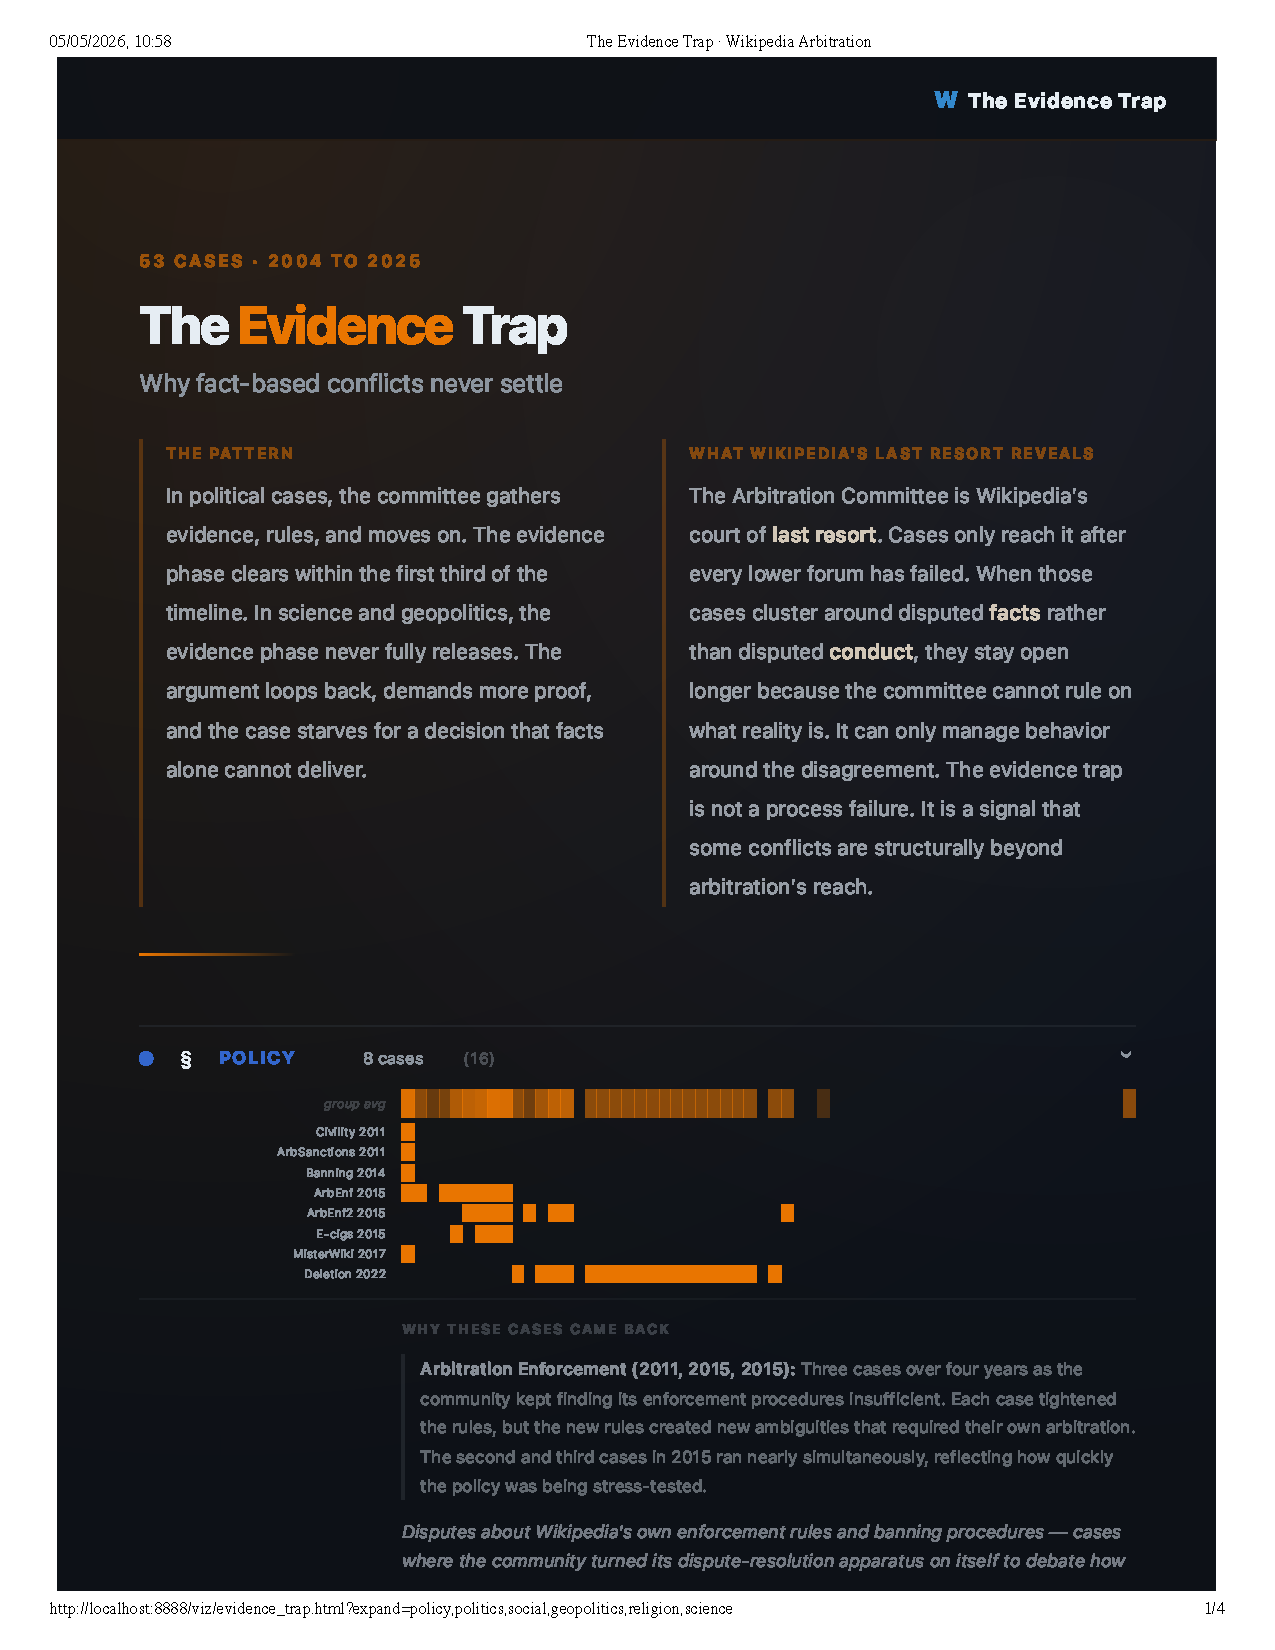
\includegraphics[width=\linewidth,height=0.88\textheight,keepaspectratio]{../static/evidence_trap.pdf}%
  }
  \caption{\small\textcolor{gray}{
    Interactive visualization of all 53 ArbCom cases grouped by dispute type
    (\href{https://observablehq.com/d/7bff75758de5a3c9}{live version}).
    Each row is a case's \textbf{group average} evidence fraction across 60 equal time windows.
    \textcolor{ev}{Orange} intensity = share of edits belonging to the evidence phase;
    dark cells = no evidence activity.
    \textbf{Fact-based groups} (Geopolitics, Science, Religion): orange persists well past the midpoint
    --- the evidence record is never considered complete.
    \textbf{Conduct-based groups} (Politics, Policy, Social): orange concentrates in the first third
    then clears --- the committee gathers what it needs, rules, and closes.
    Rows expand on click to reveal individual cases.
  }}
  \label{fig:evidence-trap}
\end{figure}
\clearpage

%----------------------------------------------------------------------------------------
%       SECTION 3
%----------------------------------------------------------------------------------------

\section{Findings}

The six group-average rows tell the story without requiring any individual case
to be opened.

\textbf{Politics and Policy clear evidence fast.}
Policy cases follow the same grammar: the evidence phase is bounded, the
committee deliberates, and a procedural ruling ends the proceedings cleanly.
Both groups deal in conduct and rule-application, questions with answers
the committee can actually deliver.

\textbf{Science and Geopolitics never release the evidence phase.}
The orange glow in the Science and Geopolitics group-average bars does not
dim after the first third of the timeline.
It persists at mid-to-high brightness well past the midpoint and in some
cases runs all the way to the end.
Climate Change returned to arbitration three times in five years.
Palestine--Israel reached the committee five times over two decades.
Each time, the evidence phase re-ignited because the underlying factual
dispute (what happened, which source is reliable, whose framing is
neutral) was not resolved by the previous ruling.

\textbf{The bottleneck is not the ruling. It is building the record.}
The proposed-decision band is almost always thin across all six groups.
Committees decide quickly once they act.
What the orange bars reveal is that in fact-based disputes,
``acting'' is perpetually deferred because the evidence record is never
considered complete.
New editors arrive, challenge previous sourcing conclusions, and the orange
phase reactivates.


%----------------------------------------------------------------------------------------
%       SECTION 4
%----------------------------------------------------------------------------------------

\section{Reflection}

I went through several iterations to come up with this picture. Originally I wanted to focus on the edits and revert "wars" for some of the longer term topics. The difficulty ended up in the "so what", and it was too easy to have the reader get caught in the specifics of each case rather than seeing the structure. You don't need to know the difference between "work-shopping" and "evidence" or that some cases end up snowballing and being about way more than they started on. I had trouble teasing out that pattern, so I did what I could to really distill down to the "evidence" of each case.


Two things I would improve.

1) the group-average row uses a simple arithmetic mean across all 60
windows, which can obscure the bimodal signal visible in Religion: some cases
clear the evidence phase early and some never do, and those two patterns
average into a flat middle that undersells the actual spread.
A small density strip alongside the mean bar would show whether the group
average is tight or hiding two sub-populations.\\

2) There doesn't seem to be a real sense of scale of editor involvement or how long some of these things took. This was by design, as they were distracting from the main point, but there is something there that should be revisited.

Thank you for a great Semester! I look forward to your feedback.


\section{AI Disclosure}
I did help use the Claude code to help draft the code for this viz. All prompts and data are available on request.


\bigskip
{\sloppy\noindent\textcolor{ev}{\rule{\linewidth}{0.4pt}}
\smallskip
\noindent\small\textbf{Repositories:}
\begin{itemize}
  \itemsep0pt
  \item \textbf{Capstone pipeline} (data collection \& processing):
    \href{https://github.com/rah-ds/Wikipedia_Dispute_Models}%
         {github.com/rah-ds/Wikipedia\_Dispute\_Models}
    (private -- email \href{mailto:rah5ff@virginia.edu}{rah5ff@virginia.edu} to request access)
  \item \textbf{Data visualization coursework} (this assignment \& all visualizations):
    \href{https://github.com/rah-ds/Data_Viz_Class}%
         {github.com/rah-ds/Data\_Viz\_Class}
  \item \textbf{Interactive visualization} (Observable notebook):
    \href{https://observablehq.com/d/7bff75758de5a3c9}%
         {observablehq.com/d/7bff75758de5a3c9}
\end{itemize}}

\end{document}
